\documentclass{article} % Default font size and left-justified equations
% \documentclass{book}

\usepackage[
  margin=0.7in,
  % includefoot,
  % footskip=30pt,
]{geometry}

\usepackage{natbib}
\usepackage{enumitem}
\usepackage{amsmath,amsfonts}
\usepackage{graphicx}
\usepackage{framed}
\usepackage{subcaption}
\usepackage[T1]{fontenc}%
\usepackage[utf8]{inputenc}%
\usepackage{mathrsfs}%
\usepackage{amssymb}%
\usepackage{amsthm}%
\usepackage{graphicx}
\usepackage{hyperref}
\usepackage{environ}
\usepackage{framed}
\usepackage{mdframed} 
\usepackage{wrapfig} 
\usepackage{booktabs}
\usepackage{tabularx} 
\usepackage{array}
\usepackage[font=small]{caption} 
\usepackage{xspace}  
\usepackage[osf,sc]{mathpazo}
\usepackage{pbox}
\usepackage{listings}
\usepackage{tikz}
\usepackage{bm}
\usepackage[strict]{changepage}
\usepackage{mleftright}
\usepackage{appendix}%
\usepackage[all]{xy} 
\setcounter{tocdepth}{3}
\setcounter{secnumdepth}{3}
\usepackage[ruled,vlined]{algorithm2e}
\usepackage{framed}
\usepackage{wrapfig}
\usepackage{pythonhighlight}
\usepackage{tikz}
\usetikzlibrary{arrows}
\usetikzlibrary{arrows.meta}
\usetikzlibrary{shapes.geometric}
\usetikzlibrary{positioning, arrows, automata, calc}
\usepackage{transparent}
\usepackage[many]{tcolorbox}
\usepackage{tikz}
\usetikzlibrary{shapes.geometric}
\usetikzlibrary{positioning, arrows, automata, calc}

\newtcolorbox[]{your_solution}[1][]{
    % breakable,
    enhanced,
    nobeforeafter,
    colback=white,
    title=Your Answer,
    sidebyside align=top,
    box align=top,
    #1
}
\newcommand{\mybox}[1]{
\noindent
\fbox{\parbox{0.955\textwidth}{%
\noindent\texttt{#1}
}
}
}

\newcommand{\filler}{ . . . . . }
\newcommand{\choice}{\hspace{0.5cm}$\square$}
\newcommand{\identity}{\mathbf{I}} 
\newcommand{\paran}[1]{\left( #1 \right)}

%% PLEASE USE THESE MACROS WHEN WRITING THE SOLUTIONS 
\newcommand{\solution}[1]{\textcolor{blue}{Answer: \em #1}
} % show
%\newcommand{\solution}[2]{#2} % hide

\newcommand{\extracredit}{{\color{purple}\textbf{Extra Credit:}}}

\newcommand{\additionalNotes}{
\noindent\textbf{How to hand in your written work:} via MyClasses.  \\ 


\noindent\textbf{Collaboration:} Make certain that you understand the course collaboration policy, described on the course website. 
You may discuss the homework to understand the problems and the mathematics behind the various learning algorithms, but you are \textcolor{red}{\textbf{not allowed to share problem solutions with any other students. You must write the solutions \textbf{individually}}}. \\ 

\noindent\textbf{Typesetting:} 
We strongly recommend typesetting your homework, especially if you have sloppy handwriting. 
% We recommend using LaTeX, but you are welcome to use whatever program and/or markup language you like. 
We will provide a LaTeX template for homework solutions. Type your answers into the corresponding solution field under each question.
}

\title{ \Large COSC490LLMs }
\date{\\ 
\normalsize Name: \_\_\_\_\_\_\_\_\_Kyle Tranfaglia\_\_\_\_\_\_\_\_\_\_\_\_\_\_\_\_\_\_\_\_\_\_\_\_\_\_\_\_\_\_\_    \\ 
Collaborators, if any: \_\_\_\_\_\_Dustin O'Brien (Math discussion)\_\_\_\_\_\_\_\_\_\_\_\_\_\_ \\ 
Sources used for your homework, if any: \_\_\_\_ChatGPT (numpy and pytorch documentation and examples/explainations) \_\_\_\_\_\_\_\_\_\_\_\_\ 
}

\newcommand{\todo}{\textcolor{blue}{\textbf{TODOs}}}



\usepackage{macros}

\author{
\Large
Homework 2: Language modeling + count-based LMs \\ \Large+ preliminaries to neural networks 
}


\begin{document}

\maketitle 

\noindent\fbox{
    \parbox{\textwidth}{
        \textbf{Homework goals:} After completing this homework, you should be able to be comfortable with various foundational concepts related to our course.   
         Specifically, we hope you will gain the followings: 
        \begin{itemize}
            \item Get more comfortable with linear algebra, specifically gradients and Jacobians! 
            \item Gain a better grasp of count-based language models! 
            \item Get comfortable with activation functions such as the Softmax function!
            \item Know how to develop your own classifier! 
        \end{itemize}
    }
}

\vspace{0.5cm}

\noindent\textbf{How to hand in your written work:} Via MyClasses as before. 

\clearpage

\section{Concepts, intuitions and big picture}
% \subsection{Training Neural Nets}

\begin{enumerate}
    \item The $n$-gram models we've shown make the $n$-th order Markov assumption, i.e. that the distribution of words depends only on the previous $n - 1$ words. What properties of language will it not capture? Discuss (briefly) several distinct ways in which this assumption is false for natural language.\\
    \solution{For natural language, this assumption is false as it exhibits multiple properties that this restraining assumption fails to capture. First, linguistic structures tend to have long-ranging dependencies such as subject-verb agreement. Words early in the sentence tend to dictate tense and the subject can be placed in the beginning of a sentence but the corresponding verb may appear later. Second, context and meaning tends to be coherent and builds or solidifies among sentences. Thus, an n-gram model will likely fail to capture topic consistency across a section of sentences. Third, n-gram models will not capture anything beyond simple (and sequential) dependencies as complex sentences involve intricate relationships and structures. Finally, idoms and some slang, especially those that introduce metaphoric language will likely be problematic for an n-gram model as a phrase like "A piece of cake" may be interpreted literally given recent language opposed to larger structures.   }
    \item  Follow-up to previous question: Despite the Markov assumption, $n$-gram models are remarkably good at predicting the next word. Discuss why this might be. What information is in the previous word(s) that makes these models perform so surprisingly well? In particular, what kinds of grammatical information do they capture?\\
    \solution{Although there are instances that n-grams may fail capture certain properties, it is overall successful as language is highly structured with local dependencies. In fact, many grammatical structures involve short-range dependencies with many pairings such as prepositions and verb-tense agreement. There is also a lot of common phrases and word parings that are significant to everyday conversation. Domain-specific training can help improve predictions even more as certain words are much more probable for certain language formats and uses. This leads into one of the biggest reasons for success: statistical regularities. Enough data allows models predict words by probabilities given context and is guided by crucial sentence reliant words such as "the," "is," "a," and "of," although it remains useful even if the probabilities are not high or overwhelmingly clear. } 
    \item Explain how are perplexity and cross-entropy loss related? \\ 
    \solution{Perplexity and cross-entropy are closely related metrics for evaluating language models. Cross-entropy measures how well the predicted probability distribution aligns with the true data distribution, with lower values indicating better performance. It is defined as the negative average log probability of the correct words. Perplexity is the exponentiation of cross-entropy, representing the number of choices the model is uncertainly considering between when predicting the next word. A lower cross-entropy directly leads to a lower perplexity such that they are perfectly correlated, and a confident and accurate model is produced in successful cases. Thus, minimizing cross-entropy also minimizes perplexity (and vice-versa), making the model more efficient in generating grammatical and contextual language. }
    \item For a vocabulary of $|V|$ words, what would you expect perplexity to be if your model predictions were completely random? Compute the corresponding cross-entropy loss for $|V| = 2000$ and $|V| = 10000$, and keep this in mind as a baseline.\\
    \solution{If a language model's predictions are completely random, each word in the vocabulary has an equal probability of being chosen. Thus, the probability of any word is $P(w) = \frac{1}{|v|}$. With this, we can find cross-entropy which for a uniform distribution is $H(P) = -\sum P(w) \log_2 P(w)$. Since all words have equal probability, we can simplify this with $P(w) = \frac{1}{|v|}$ to $H(P) = -\log_2 \left( \frac{1}{|V|} \right) = \log_2 |V|$. Finally, we use the Perplexity equation, $PP = 2^H(P)$ to get that $PP = 2^{\log_2 |V|} = |V|$. \\ \\ As for $|V| = 2000$ and $|V| = 10000$, we get that $H(P) = \log_2 2000 \rightarrow PP = 2000$ and  $H(P) = \log_2 10000 \rightarrow PP = 10000$.}

    \item Which of these are reasons for the recent wave of neural networks taking off? (check the options that apply.) \\ 
        \hspace{1cm}\checkmark{} We have access to a lot more computational power.\\
        \hspace{1cm}\choice{} Neural Networks are a brand new field.\\
        \hspace{1cm}\checkmark{} We have access to a lot more data.\\
        \hspace{1cm}\checkmark{} There has been significant improvements in benchmarks in speech recognition and NLP.\\
        \solution{}
    \item What does a neuron compute? \\ 
        \hspace{1cm}\choice{} A neuron computes an activation function followed by a linear function ($z = Wx + b$)\\
        \hspace{1cm}\checkmark{} A neuron computes a linear function ($z = Wx + b$) followed by an activation function.\\
        \hspace{1cm}\choice{} A neuron computes a function $g$ that scales the input $x$ linearly ($Wx + b$).\\
        \hspace{1cm}\choice{} A neuron computes the mean of all features before applying the output to an activation function.\\
        \solution{}

    \item  What is the point of applying a Softmax function to the logits output by a sequence classification model? \\ 
        \hspace{1cm}\checkmark{} It softens the logits so that they're more reliable. \\ 
        \hspace{1cm}\checkmark{} It applies a lower and upper bound so that they're understandable. \\ 
        \hspace{1cm}\checkmark{} The total sum of the output is then 1, resulting in a possible probabilistic interpretation.\\
        \solution{}
    
\end{enumerate}

\clearpage

\section{Linear Algebra Recap}
\subsection{Gradients}
Consider the following scalar-valued function: 
$$
    f(x, y, z) = x^2y + \text{sin}(z+6y). 
$$

\begin{enumerate}
    \item Compute partial derivatives with respect to $x$, $y$ and $z$. \\
    \solution{\\ $\frac{\partial f}{\partial x} = 2xy$ \\ $\frac{\partial f}{\partial y} = x^2 + 6cos(z + 6y)$ \\ $\frac{\partial f}{\partial z} = cos(z + 6y)$ \\ 
    \[
    \nabla f(x, y , z) =
    \begin{bmatrix}
    \frac{\partial f}{\partial x} \\
    \frac{\partial f}{\partial y} \\
    \frac{\partial f}{\partial z}
    \end{bmatrix}
    \rightarrow
    \begin{bmatrix}
    2xy \\
    x^2 + 6\cos(z + 6y) \\
    \cos(z + 6y)
    \end{bmatrix}
    \]}
    
    \item We can consider $f$ to be a function that takes a vector $\theta \in \reals^3$ as input, where $\theta = [x, y, z]^\top$. 
    Write the gradient as a vector and evaluate it at $\theta = [3, \pi/2, 0]^\top$.\\
    \solution{\[
    \nabla f(3, \pi/2, 0)  =
    \begin{bmatrix}
    2(3)(\pi/2) \\
    3^2 + 6\cos(0 + 6(\pi/2) \\
    \cos(0 + 6(\pi/2)
    \end{bmatrix}
    \rightarrow
    \begin{bmatrix}
    3\pi \\
    3 \\
    -1
    \end{bmatrix}
    \]}
\end{enumerate}


%%%%%%%%%%%%%%%%%%%%%




\subsection{Gradients of vectors}

Let $\mathbf{x}, \mathbf{c} \in \reals^n$ and $\mathbf{A} \in \reals^{n \times n}$. 
For the following parts, before taking any derivatives, identify what the
derivative looks like (is it a scalar, vector, or matrix?) and how we calculate each term in the derivative. Then carefully solve for an arbitrary entry of the derivative, then stack/arrange all of them to get the final
result. 

\begin{itemize}
    \item Show that $\frac{\partial }{ \partial \mathbf{x} } \left( \mathbf{x}^\top \mathbf{c}  \right) = \mathbf{c}^\top$.\\
    \solution{The function $ \left(\mathbf{x}^\top \mathbf{c}  \right) = \mathbf{c}^\top$ is a scalar since it is the dot product of two vectors. The derivative of a scalar function with respect to a vector is a row vector. So, we can compute an arbitrary entry of the derivative, take the partial derivative with respect to $x_i$ (representing the function as a sum of entries, and then stack all the partial derivatives. \\
    $x^\top c = \sum_{j=1}^{n} x_j c_j \rightarrow \frac{\partial}{\partial x_i} (x^\top c) = \frac{\partial}{\partial x_i} \sum_{j=1}^{n} x_j c_j \rightarrow \frac{\partial}{\partial x_i} (x^\top c) = c_i \rightarrow \frac{\partial}{\partial x} (x^\top c) = [c_1, c_2, \dots, c_n] = c^\top$}
    \item Show that $\frac{\partial }{ \partial \mathbf{x} } \left( \norm{\mathbf{x}}^2_2 \right) = 2\mathbf{x}^\top$.\\
    \solution{The function $\left( \norm{\mathbf{x}}^2_2 \right)$ is a scalar since it is the magnitude of vector x, so its derivative, with respect to x should be a row vector. \\
    $x^\top x = \sum_{j=1}^{n} x_j x_j = \sum_{j=1}^{n} x_j^2 \rightarrow \frac{\partial}{\partial x_i} (x^\top x) = \frac{\partial}{\partial x_i} \sum_{j=1}^{n} x_j^2 \rightarrow \frac{\partial}{\partial x_i} (x^\top x) = 2x_i \rightarrow \frac{\partial}{\partial x} (x^\top x) = [2x_1, 2x_2, \dots, 2x_n] = 2x^\top$}
    \item Show that $\frac{\partial }{ \partial \mathbf{x} } \left( \mathbf{A} \mathbf{x} \right) = \mathbf{A}$.\\
    \solution{The derivative of an n-dimensional vector function with respect to an n-dimensional vector should result in an n x n matrix. Since Ax is an n-dimensional vector, to find the derivative, we need to determine how each component changes with respect to each x. \\ 
    $(Ax)_i = \sum_{j=1}^{n} A_{ij} x_j \rightarrow \frac{\partial}{\partial x_k} (Ax)_i = \frac{\partial}{\partial x_k} \sum_{j=1}^{n} A_{ij} x_j \rightarrow \frac{\partial}{\partial x_k} (Ax)_i = A_{ik} \rightarrow \frac{\partial}{\partial x} (Ax) = A$}
    \item Show that $\frac{\partial }{ \partial \mathbf{x} } \left( \mathbf{x}^\top \mathbf{A}  \mathbf{x} \right) = \mathbf{x}^\top (\mathbf{A} + \mathbf{A}^\top)$.\\
    \solution{The function $\left( \mathbf{x}^\top \mathbf{A}  \mathbf{x} \right)$ is a scalar, again such that it is the result of a dot product between vectors, so its derivative with respect to a vector should be a row vector. \\
    $\left( \mathbf{x}^\top \mathbf{A}  \mathbf{x} \right) = \sum_{i=1}^{n} \sum_{j=1}^{n} x_i A_{ij} x_j \rightarrow \frac{\partial}{\partial x_k} \sum_{i=1}^{n} \sum_{j=1}^{n} x_i A_{ij} x_j \rightarrow \sum_{i=1}^{n} \sum_{j=1}^{n} \frac{\partial}{\partial x_k} (x_i A_{ij} x_j) \rightarrow \frac{\partial}{\partial x_k} (x^\top A x) = \sum_{j=1}^{n} A_{kj} x_j + \sum_{i=1}^{n} A_{ik} x_i \rightarrow \frac{\partial}{\partial x} (x^\top A x) = x^\top A + x^\top A^\top$}
\end{itemize}

\paragraph{Note:}The above equations follow the \href{https://en.wikipedia.org/wiki/Matrix_calculus#Layout_conventions}{numerator layout} notation which is commonly following in linear algebra, but there are alternative notational conventions as well. 

%%%%%%%%%%%

\subsection{Jacobian}
Consider the following vector function from $\reals^3$ to $\reals^3$: 
$$
    \mathbf{f}(\boldsymbol{\theta} = [x_1, x_2, x_3]) = 
    \begin{cases}
        \text{sin}(x_1x_2x_3) \\
        \text{cos}(x_2 + x_3) \\
        \exp(-\frac{1}{2}x_3^2) \\
    \end{cases}
$$

\begin{enumerate}
    \item What is the Jacobian matrix\footnote{\url{https://en.wikipedia.org/wiki/Jacobian_matrix_and_determinant}} of $\mathbf{f}(\boldsymbol{\theta})$?\\
    \solution{Partial derivatives of $f_1 = \sin(x_1 x_2 x_3): \frac{\partial f_1}{\partial x_1} = x_2 x_3 \cos(x_1 x_2 x_3), \frac{\partial f_1}{\partial x_2} = x_1 x_3 \cos(x_1 x_2 x_3), \frac{\partial f_1}{\partial x_3} = x_1 x_2 \cos(x_1 x_2 x_3)$ \\
    Partial derivatives of $f_2 = \cos(x_2 + x_3): \frac{\partial f_2}{\partial x_1} = 0,  \frac{\partial f_2}{\partial x_2} = -\sin(x_2 + x_3), \frac{\partial f_2}{\partial x_3} = -\sin(x_2 + x_3)$ \\
    Partial derivatives of $f_3 = \exp(-\frac{1}{2} x_3^2):  \frac{\partial f_3}{\partial x_1} = 0,    \frac{\partial f_3}{\partial x_2} = 0,    \frac{\partial f_3}{\partial x_3} = -x_3 \exp(-\frac{1}{2} x_3^2)$. \\ 
    Thus, the Jacobian matrix is: $J(\mathbf{f}({\theta}) =
    \begin{bmatrix}
    x_2 x_3 \cos(x_1 x_2 x_3) & x_1 x_3 \cos(x_1 x_2 x_3) & x_1 x_2 \cos(x_1 x_2 x_3) \\
    0 & -\sin(x_2 + x_3) & -\sin(x_2 + x_3) \\
    0 & 0 & -x_3 e^{-x_3^2 / 2}
    \end{bmatrix}$}
    
    \item Evaluate the Jacobian matrix of $\mathbf{f}(\boldsymbol{\theta})$ at 
    $\boldsymbol{\theta} = [1, \pi, 0]$.\\
    \solution{$J(\mathbf{f}({\theta = [1, \pi, 0]})) =
    \begin{bmatrix}
    0 & 0 & \pi \\
    0 & 0 & 0 \\
    0 & 0 & 0
    \end{bmatrix}$}
\end{enumerate}

\clearpage


\section{$n$-gram Language Models}
\subsection{A toy $n$-gram language model}

Consider the following vocabulary, $V= \{\tt BOS, EOS, who, framed, roger, rabbit, the\}$ where \texttt{BOS} is the dummy token indicating the beginning of a sentence, and \texttt{EOS} indicates the end of a sentence. Consider the following training data:

\noindent\fbox{%
    \parbox{0.5\textwidth}{%
\noindent
\texttt{BOS who EOS \\ 
BOS who framed roger EOS \\ 
BOS roger rabbit EOS \\ 
BOS who framed roger rabbit EOS \\ 
BOS roger framed who EOS \\ 
BOS who framed the rabbit EOS \\
}}}

\begin{enumerate}
    \item Compute the following probabilities: $P(\texttt{rabbit})$, $P(\texttt{rabbit}|\texttt{roger})$, $P(\texttt{EOS}|\texttt{rabbit})$.\\
    \solution{$P(\text{rabbit}) = \frac{\text{Count}(\text{rabbit})}{\sum \text{all words}} = \frac{3}{29}$ \\
    $P(\text{rabbit} | \text{roger}) = \frac{\text{Count}(\text{roger} \to \text{rabbit})}{\text{Count}(\text{roger})} = \frac{2}{4} = \frac{1}{2}$ \\
    $P(\text{EOS} | \text{rabbit}) = \frac{\text{Count}(\text{rabbit} \to \text{EOS})}{\text{Count}(\text{rabbit})} = \frac{3}{3} = 1$}

    \item Briefly  explain what the sparsity problem is in $n$-gram language models? \\
    \solution{The sparsity problem in n-gram language models is the assignment of a probability of zero  to unseen or very rare n-grams. This happens since n-gram models estimate probabilities based on observed counts, and data is finite, languages are vast, and there exists rare strings. For example, given the data above P(rabbit|framed the) = 0 as this trigram does not appear in the dataset.}
\end{enumerate}



\clearpage

\section{Challenges of linear classifiers of sentences}
A simple way to compute a representation for a phrase $s$ is to add up the representations of the words in that phrase: $\text{repr}(s) = \sum_{w \in s} v_w$, 
where $w \in s$ are the word in  $s$ and $v_w \in \reals^d$ is the embedding for word $w$. 

\begin{enumerate}
    \item  Now, consider sentiment analysis on a phrase in which the predicted sentiments are 
        $$ f(s; \theta) = \theta \cdot \text{repr}(s), $$
        for some choice of parameters $\theta$. 
        Note that here $\theta  \in \reals^d$ and ``$\cdot$'' is the ``dot-product''. 
        Prove that in such a model, the following inequality cannot hold for any choice of $\theta$ and word embeddings: 
        \begin{align*}
            f(\texttt{good}; \theta)  > f(\texttt{not good}; \theta)    \\ 
            f(\texttt{bad}; \theta)  < f(\texttt{not bad}; \theta)
        \end{align*}
        Thereby, showing the inadequacy of this model in capturing negations.\footnote{Question credit: ``Introduction to Natural Language Processing'' by J. Eisenstein.} \\ 
    \solution{\begin{align*}
    f(\text{good}; \theta) &= \theta \cdot v_{\text{good}}, \\
    f(\text{not good}; \theta) &= \theta \cdot (v_{\text{not}} + v_{\text{good}}), \\
    f(\text{bad}; \theta) &= \theta \cdot v_{\text{bad}}, \\
    f(\text{not bad}; \theta) &= \theta \cdot (v_{\text{not}} + v_{\text{bad}}).
    \end{align*} \\ 
    $f(\text{good}; \theta) > f(\text{not good}; \theta) = \theta \cdot v_{\text{good}} - \theta \cdot v_{\text{good}} > \theta \cdot v_{\text{not}} = 0 > \theta \cdot v_{\text{not}}$ \\
    $\theta \cdot v_{\text{bad}} < \theta \cdot (v_{\text{not}} + v_{\text{bad}}) = \theta \cdot v_{\text{bad}} - \theta \cdot v_{\text{bad}} < \theta \cdot v_{\text{not}} = 0 < \theta \cdot v_{\text{not}}$ \\
    Thus, the two inequalities require that $\theta$ be both positive and negative simultaneously such that we reach a contradiction. Therefore, the following inequality cannot hold for any choice of $\theta$ and word embeddings.}
   
    \item  Consider a slight modification to the previous predictive model: 
        $$ 
            f(s; \theta) = \theta \cdot \text{ReLU}\big( \text{repr}(s) \big), 
        $$
        where ReLU (rectified linear function) is defined as: 
        $$
            \text{ReLU}(x) = 
            \begin{cases}
                x & \text{ if } x \geq 0  \\ 
                0 & \text{ if } x < 0.
            \end{cases}
        $$
        Given this choice of predictive function, show that it is possible to satisfy the above inequalities for some choice of $\theta$. 
        \textbf{Hint:} Show there exists parameters $\theta$ and word embeddings $v_\texttt{good}$, $v_\texttt{bad}$ and $v_\texttt{not}$ that the inequalities are satisfied. \\ 
    \solution{Assume the embeddings: \\
    $v_{\text{good}} = \begin{bmatrix} 0 \\ 3 \end{bmatrix}, \quad v_{\text{bad}} = \begin{bmatrix} 3 \\ -2 \end{bmatrix}, \quad v_{\text{not}} = \begin{bmatrix} 1 \\ -2 \end{bmatrix}$ \quad where $\theta$ is positive\\
    For "good": \\ $\text{ReLU}(v_\text{good}) = \begin{bmatrix} 0 \\ 3 \end{bmatrix}$ \\
    For "not good": \\$\text{ReLU}(f(\text{not good}; \theta)) = \text{ReLU}(v_\text{not} + v_\text{good}) = \text{ReLU}(\begin{bmatrix} 1 \\ -2 \end{bmatrix} + \begin{bmatrix} 0 \\ 3 \end{bmatrix}) = \begin{bmatrix} 1 \\ 1 \end{bmatrix}$ \\
    So, we get that $(f(\text{not good}; \theta)) < (f(\text{good}; \theta))$ as $\theta \cdot \begin{bmatrix} 1 \\ 1 \end{bmatrix} < \begin{bmatrix} 0 \\ 3 \end{bmatrix} \cdot \theta$ \\
    For "bad": \\ $\text{ReLU}(v_\text{bad}) = \begin{bmatrix} 3 \\ 0 \end{bmatrix}$ \\ 
    For "not bad": \\ $\text{ReLU}(f(\text{not bad}; \theta)) = \text{ReLU}(v_\text{not} + v_\text{bad}) = \text{ReLU}(\begin{bmatrix} 1 \\ -2 \end{bmatrix} + \begin{bmatrix} 3 \\ -2 \end{bmatrix}) = \begin{bmatrix} 4 \\ 0 \end{bmatrix}$ \\
     So, we get that $(f(\text{bad}; \theta)) < (f(\text{not bad}; \theta))$ as $\theta \cdot \begin{bmatrix} 3 \\ 0 \end{bmatrix} < \begin{bmatrix} 4 \\ 0 \end{bmatrix} \cdot \theta$ \\
     Thus, we satisfy both inequalities, as multiplying the vectors by any positive $\theta$ with the given word embeddings supports both inequalities.}
    \item Given the above result, explain (in 1-2 sentence) why the use of neural networks (which have more complexity than linear models)
    \\
    \solution{Neural networks introduce non-linearity (ReLU), allowing them to model more complex relationships between words and sentiment. Unlike linear models, which struggle with contradictions as shown above, neural networks can selectively activate or suppress certain word contributions, enabling them to capture nuanced meanings and context-dependent sentiment shifts.}
\end{enumerate}


% \newpage %%%%%%%%%%%%%%%%%%%%%%%%%%%%%%%%%%%%%%%%%%%%%%%%%%%%%%%%%%%%%%%%%%%%%%%%%%%%%%%%%%

\section{Softmax function}
\label{sec:softmax}
Remember  the Softmax functions from the class: 
$$
    \text{Softmax: } \sigma(\mathbf{z}) \triangleq [\sigma(\mathbf{z})_1, \hdots, \sigma(\mathbf{z})_K] \; \text{s.t.} \;  \sigma(\mathbf{z})_i = \frac{e^{z_i}}{\sum_{j=1}^K e^{z_j}} \ \ \text{ for } i = 1, \dotsc, K \text{ and } \mathbf{z} = (z_1, \dotsc, z_K)
$$

\begin{enumerate}
    \item  Prove that Softmax is invariant to constant offsets in the input, i.e., for any input vector \label{subsec:5.1}
    $\mathbf{z}$ and any constant $c$,
    $$
        \sigma(\mathbf{z}) = \sigma(\mathbf{z} + c) 
    $$
    \textbf{Pro tip: } We make use of this property in practice to increase the numerical stability of our models. 
    Specifically, using  $c = - \max_{i \in \set{1 ... K}} z_i$, i.e. subtracting its maximum element from all elements of $\mathbf{z}$ would prevent numerical instability  due to large values. \\
    \solution{Lets consider the following addition of a constant to the Softmax function, $\sigma(\tilde{z})_i = \frac{e^{\tilde{z}_i}}{\sum_{j=1}^{K} e^{\tilde{z}_j}}
    = \frac{e^{z_i + c}}{\sum_{j=1}^{K} e^{z_j + c}}$ \\
    Now we factor out $e^c \rightarrow \sigma(\tilde{z})_i = \frac{e^{z_i} e^c}{e^c \sum_{j=1}^{K} e^{z_j}} \rightarrow \sigma(\tilde{z})_i = \frac{e^{z_i}}{\sum_{j=1}^{K} e^{z_j}} = \sigma(z)_i$ \\ Thus, we show that $\sigma(z + c) = \sigma(z),$ proving that the Softmax function is invariant to constant offsets}
    
    \item Softmax maintains the relative order of the elements in $\mathbf{z}$. In particular, show that the largest index is intact after applying Softmax: 
    $$
        \argmax_{i \in \set{1 ... K}} z_i =  \argmax_{i \in \set{1 ... K}}  \sigma(\mathbf{z})_i
    $$
    \solution{Let $i^*$ be the index of the largest element in z. \\ $i^* = \arg \max_{i \in \{1, \dots, K\}} z_i $ \\ Adding $e^x$ to both sides, we preserve its order $i^* = \arg \max_{i \in \{1, \dots, K\}} z_i$ \\ Then we divide by the same denominator to preserve the ordering $\sigma(z)_{i^*} = \frac{e^{z_{i^*}}}{\sum_{j=1}^{K} e^{z_j}} \geq \sigma(z)_j, \quad \forall j$ \\ Thus, $\arg \max_{i} z_i = \arg \max_{i} \sigma(z)_i$, proving that Softmax maintains the relative ordering of z, and preserves the index of its largest element.}
    \item Define the Sigmoid function as follows: 
    $$
        \text{Sigmoid: } S(x) \triangleq \frac{1}{1 + e^{-x}} = \frac{e^x}{e^x + 1}=1-S(-x). 
    $$
    Prove that Softmax is equivalent to the Sigmoid functions when the number of possible labels is two: $K=2$. Specifically: 
    $$ \sigma_1([z_1, z_2]) = S(z_1 - z_2) $$
    \\
    \solution {defining the Softmax function for two labels (k = 2), we get that $\sigma_1([z_1, z_2]) = \frac{e^{z_1}}{e^{z_1} + e^{z_2}}, \sigma_2([z_1, z_2]) = \frac{e^{z_2}}{e^{z_1} + e^{z_2}}$ \\
    Let $\Delta z = z_1 - z_2$. Then we can write the function as the following, \\
    $\sigma_1([z_1, z_2]) = \frac{e^{z_1}}{e^{z_1} + e^{z_2}} = \frac{e^{z_2} \cdot e^{(z_1 - z_2)}}{e^{z_2} \cdot (1 + e^{(z_1 - z_2)})} = \frac{e^{(z_1 - z_2)}}{1 + e^{(z_1 - z_2)}}$ With the definition of the Sigmoid function $S(x) = \frac{e^x}{1 + e^x}$, we can conclude that $\sigma_1([z_1, z_2]) = S(z_1 - z_2)$. Thus, we prove that when $k = 2$, the Softmax function reduces to the Sigmoid function.}
    
   
\end{enumerate}

\newpage
    



\section{Programming}
In this programming homework, we will
\begin{itemize}
    \item build a simple count-based (n-gram) language model.
    \item implement your own gradient descent optimization for the classifier you built in homework 1.
\end{itemize}


\noindent \paragraph{Skeleton Code and Structure:}
The code base for this homework can be found at MyClasses/Files under the \texttt{hw2} directory. Your task is to fill in the missing parts in the skeleton code, following the requirements, guidance, and tips provided in this pdf and the comments in the corresponding .py files.
The code base has the following structure:
\begin{itemize}
    \item \texttt{ngram\_lm.py} implements a n-gram language model on a subset of Wikipedia. 
    \item \texttt{gradient\_descent.py} reuse the sentiment classifier on movie reviews you implemented in homework 1, with additional requirements to implement manual softmax, cross-entropy loss, and gradient updates.
    \item \texttt{main.py} provides the entry point to run your implementations in both \texttt{ngram\_lm.py} and \texttt{backprop.py}.
    \item \texttt{hw2.md} provides instructions on how to setup the environment and run each part of the homework in \texttt{main.py}
\end{itemize}


\noindent \todo{} ---
Your tasks include
1) generate plots and/or write short answers based on the results of running the code; 2) fill in the blanks in the skeleton to complete the code. We will explicitly mark these plotting, written answer, and filling-in-the-blank tasks as \todo{} in the following descriptions, as well as a \textcolor{blue}{\texttt{\textbf{\#~TODO}}} at the corresponding blank in the code. \\

\noindent \todo{} (Copy from your HW1). We are reusing most of the \texttt{model.py} from homework 1 as the starting point for the \texttt{gradient.py} - you will see in the skeleton that they look very similar. Moreover, in order to make the skeleton complete, for all the \textcolor{blue}{\texttt{\textbf{\#~TODO (Copy from your HW1)}}}, please fill in the blank below them by copying and pasting the corresponding implementations you wrote for homework 1 (i.e. the corresponding \textcolor{blue}{\texttt{\textbf{\#~TODO}}} in homework 1.)

\noindent \paragraph{Submission:} Your submission should contain two parts: 1) plots and short answers under the corresponding questions below; and 2) your completion of the skeleton code base, in a \texttt{.zip} file

\subsection{Count-based LMs}
\label{subsubsec:count-based lms}
In the lecture, we have learned language modeling as building probabilistic distribution (marginal and joint) over language. Moreover, we can estimate such distributions (e.g. $\Pr(X_t|X1, \cdots, X_{t-1})$) by \textit{counting}. For example $$\Pr(\textrm{mat} | \textrm{the cat sat on the}) \approx \frac{\textrm{count}(\textrm{"the cat sat on the mat"})}{\textrm{count}(\textrm{"the cat sat on the"})} $$
We are going to implement such a count-based LM, i.e. n-gram language model.

\subsubsection{Data Loading}
We will use (a subset of) the \href{https://huggingface.co/datasets/wikitext}{WikiText} dataset for building the n-gram LM. The WikiText language modeling dataset is a collection of over 100 million tokens extracted from the set of verified Good and Featured articles on Wikipedia. 
Spend a few minutes reading a few examples on Huggingface to get a better sense of what this dataset looks like. We will use Huggingface's datasets library to download this dataset locally. For efficiency, we only use the first $1\textrm{e}5$ training samples to create our LM.\\\

\noindent Read the \texttt{load\_data} function in \texttt{ngram\_lm.py} for how we obtain the data.

\subsubsection{Preprocessing: Sentence Split and Tokenization}
As you have seen, each data sample consists of a Wikipedia paragraph. To perform our n-gram counting, we need first split each paragraph into sentences \footnote{we count n-gram status within sentence boundary} and then each sentence into a sequence of tokens (i.e. \textit{tokenization} that we introduced in homework 1).
In particular, we will use \href{https://aclanthology.org/W07-0733/}{an algorithm} by Philipp Koehn for sentence splitting; and use a \textit{sub-word tokenizer} for tokenization. For now, we are using an existing sub-word tokenizer of an existing model from the Huggingface library, but in the future, we will also build our own tokenizer.

A \textit{Sub-word tokenizer} which, as it should be clear from the name, splits each sentence into units smaller than words, based on their frequency. For example, the word "Potentials" is broken into four sub-words: `Po', '\#\#ten', '\#\#tial', '\#\#s'`, where `\#\#` is a special symbol indicating that the sub-word is in the middle of a word.


Sub-word tokenization might initially seem like a bad idea since we are breaking up the word. But it brings it several benefits.
\begin{itemize}
    \item Handling Out-of-Vocabulary (OOV) words: Sub-word tokenization allows the representation of rare or unseen words as a combination of sub-words or tokens that have been seen in the training data, thus reducing the OOV problem.
    \item Improved vocabulary size: It allows for a more compact vocabulary size, reducing the size of the language model, and increasing its efficiency.
    \item Better language model performance: Sub-word tokenization results in a better representation of morphologically rich languages, where words are formed by combining roots and affixes, leading to improved language model performance.
    \item Cross-lingual compatibility: Sub-word tokenization is language-agnostic, and models trained on sub-word tokens from one language can be applied to other languages, improving cross-lingual compatibility.
    
\end{itemize}

How are sub-tokenizers built? We will delve into that in a few weeks! For now, we will just use them!
\\\\
\noindent Read the \texttt{sentence\_split\_and\_tokenize\_demo} for how exactly an \texttt{wikitext} paragraph is converted into sentences and then tokens.

\subsubsection{Build the N-gram LM: Let's Count!}
\noindent\todo{}: read the \texttt{create\_ngrams} function which iteratively processes each paragraph and counts the n-gram statistics, and completes the following lines under three \textcolor{blue}{\texttt{\textbf{\#~TODO}}}s:
\begin{itemize}
    \item tokenize the words in the sentence: that takes in a \texttt{sentence} and convert it into \texttt{tokens} as a list of tokens with the tokenizer. \\
    \textbf{Hint}: check out how to do tokenization in sentence\_split\_and\_tokenize\_demo
    \item count n-gram statistics over each list of tokens, record them in
    \begin{itemize}
        \item \texttt{ngrams}: the \texttt{Counter} for n-grams count
        \item \texttt{ngram\_context}: the \texttt{Counter} for context (i.e. (n-1)-grams) 
        count
        \item \texttt{next\_word\_candidates}: the \texttt{Dictionary} that keeps track of all possible candidate next tokens given the context, i.e. all tokens that, concatenated with the (n-1)-gram context, constitutes an n-gram that exists in the data. 
    \end{itemize}
    for all the \texttt{Counter} and \texttt{Dictionary}, use \texttt{tuple} of n-gram or (n-1)-gram tokens as the keys. \\
    \textbf{Hint}: also check the corresponding comments in the code for specific requirements
    \item computes the estimated probability of the next word (token) given the context. \\\textbf{Hint}: use the formula in \autoref{subsubsec:count-based lms}, and also the corresponding comments in the code
\end{itemize}
Finally, the \texttt{next\_word\_pred} returned from the \texttt{create\_ngrams}, will record for each (n-1) gram context, the most probable next word continuation. For this homework, we will set $n=3$ so that to build a \textit{trigram} language model.

\subsubsection{Visualize the N-gram distribution}
\todo{}: Complete the \texttt{plot\_next\_word\_prob} function in \texttt{ngram\_lm.py}, and run \texttt{run\_ngram} in \texttt{main.py} to plot the top-10 most probable next token given an input context. Paste the two plots for the two given contexts (provided in \texttt{run\_ngram}), and describe in 2-3 sentences your findings. \\
\textbf{Hints}:
\begin{itemize}
    \item you can check out \href{https://www.geeksforgeeks.org/bar-plot-in-matplotlib/}{this tutorial} about how to plot bar chart with \href{https://matplotlib.org/stable/api/_as_gen/matplotlib.pyplot.bar.html}{matplotlib}.
    \item read the comments in the code carefully for more info about the input.
\end{itemize}
\noindent {\color{red}{your plots and answer:}}\\
% uncommment the following lines to add your figures
\begin{figure}[h] 
   \centering
   \subfloat[top 10 next words of "move to"]{
       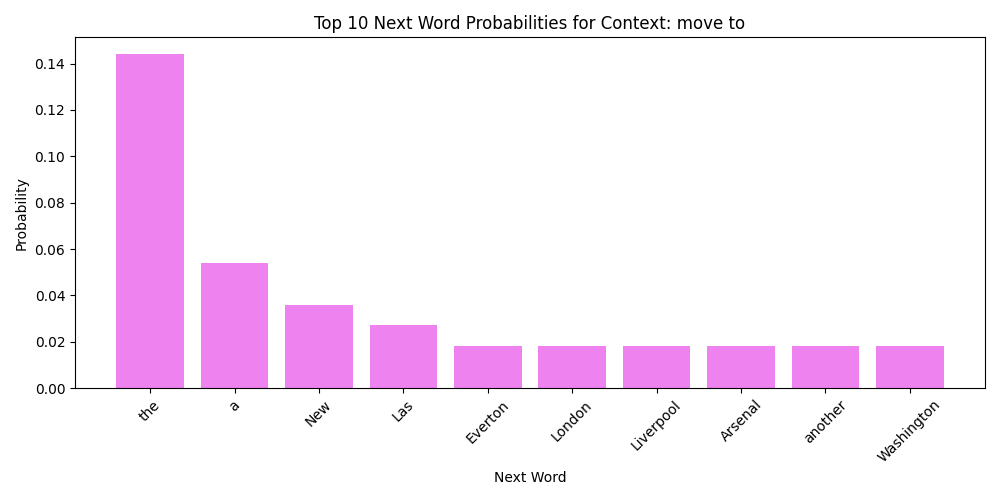
\includegraphics[width=0.45\textwidth]{ngram_context1.png}
       }
   \hfill
   \subfloat[top 10 next words of "the news"]{
       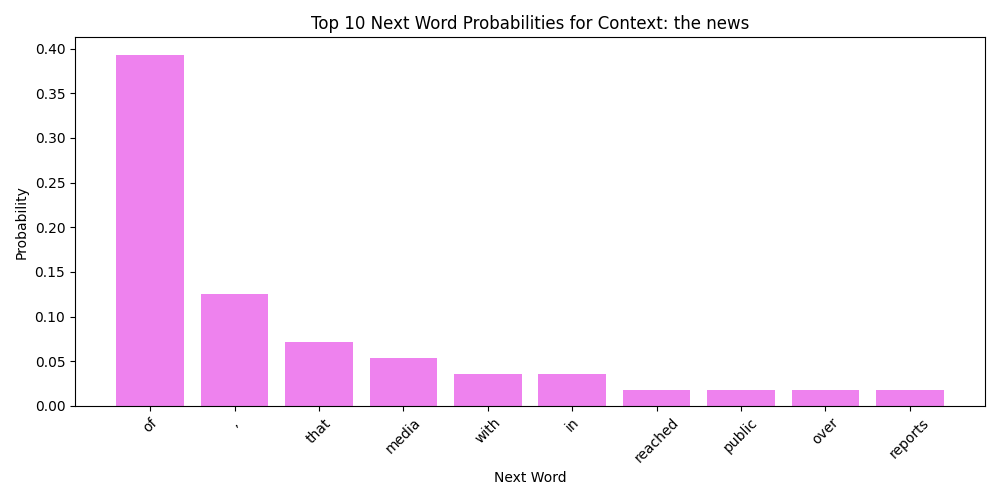
\includegraphics[width=0.45\textwidth]{ngram_context2.png}
       \label{fig:b}
       }
   \caption{The probabilities of top 10 next words of two bi-gram contexts}
\end{figure}

\noindent\solution{For the given context "move to," the top ten probabilities show a highly probably word, "the" being at over 14 percent while the next word "a," is less that half at around 6 percent. From here, the probabilities decrease linearly until the fifth word where the distribution then becomes uniform. For "the news," the probability distribution is similar with "of" being the most probably at nearly 40 percent with a falling off for the second word followed by a linear decline and then a uniform distribution. It is intereseting toi not that the second most probably word is the character "`".}

\subsubsection{Generation: Sample from the LM}
Now that we have built our LM, given any prefix\footnote{in our case of trigram LM, we require the prefix to have $\geq2$ tokens}, we can sample from the LM to generate a full completion. Specifically, at each timestamp, we take the last (n-1) tokens from the prefix as the context and query our LM to get the most probable next token, append it to the prefix, and continue until we sample the stop token our the maximum length is reached. 

This sampling procedure is called greedy decoding, as we take the most probable next token each step, there are a few other sampling strategies like beam search \citep{meisteretal2020beam}, top-k, and top-p sampling \citep{holtzman2019curious}. Similarly, we will get to them soon.
\\\\
\noindent Read the \texttt{generate\_text} function in \texttt{ngram\_lm.py} for details of the generation process described above.
\\\\
\noindent \todo{}: Run \texttt{run\_ngram} in \texttt{main.py} and paste the completion of the two given prefixes (provided in \texttt{run\_ngram}), and describe in 2-3 sentences your findings.
\\
\solution{\\Completion 1: According to the report, the first time in the United States, and the other hand, the first time in the United States, and the other hand, the first time\\
Completion 2: The president of the association ' s " The One I Love You ' re not here to Connacht side of the game ' s " The One I Love You ' re not\\
Findings: Given each generated text with the starting prompts, we can identify issues with the LM and its utilization of a greedy decoding. Since the most probable token is taken for each step, we tend to not only get very incomplete sentences that have poor flow and nonsensical structure, but there model gets stuck generating loops of the same sections of text as the next, token given the context, remains the same.}

\subsection{Optimizing the Sentiment Classifier with (Stochastic) Gradient Descent}
In the second part of this programming homework, we will revisit the sentiment classifier we built in the last homework. Instead of relying on the PyTorch built-in loss functions, gradient calculations, and weights optimization, we will delve into them and implement our own version!

\subsubsection{Reuse Your HW1 Implementation}
\todo{} (Copy from your HW1): for all the \textcolor{blue}{\texttt{\textbf{\#~TODO (Copy from your HW1)}}} in \texttt{gradient\_descent.py}, please fill in the blank below them by copying and pasting the corresponding implementations you wrote for homework 1 (i.e. the corresponding \textcolor{blue}{\texttt{\textbf{\#~TODO}}} in the \texttt{model.py} in homework 1).

\subsubsection{Softmax Function}
Remember the \href{https://pytorch.org/docs/stable/generated/torch.nn.CrossEntropyLoss.html}{nn.CrossEntropyLoss} we used in homework 1, it can be further decomposed into that 1) normalize the real-value scores of each class (e.g. the logits) into a probability distribution
using softmax function, and calculate the cross entropy loss of this probability distribution against the ground truth binary distribution (In practice, PyTorch instead provides the combination of \href{https://pytorch.org/docs/stable/generated/torch.nn.LogSoftmax.html#torch.nn.LogSoftmax}{LogSoftmax} with \href{https://pytorch.org/docs/stable/generated/torch.nn.NLLLoss.html#torch.nn.NLLLoss}{negative log likelihood loss}).  We will first implement the softmax function, which you have been familiar with in the lecture, and \autoref{sec:softmax}.
\\\\
\noindent \todo{}: Complete the \texttt{softmax} function of the \texttt{SentimentClassifier} class in \texttt{gradient\_descent.py}. Note: you must implement the optimized for numerical stability version described in the \textbf{Pro tip} in \autoref{subsec:5.1} of \autoref{sec:softmax}.
\\
\noindent \textbf{Hint}: check the comments in the code for specific input-output requirements.
\\
A correct implementation should pass the \texttt{test\_softmax} in \texttt{gradient\_descent.py}.
\\\\
\noindent With the softmax function, we turn our neural network into a classifier that assigns a probability distribution over the 2 sentiment classes. Specifically, denoting our input feature vector as $\mathbf{x}$, the \texttt{nn.Linear} layer transforms $\mathbf{x}$ into a \textbf{logit score} vector $\mathbf{z}$ using a weight matrix $W$ and a bias vector $\mathbf{b}$:

$$
    \mathbf{z} = \mathbf{x} W + \mathbf{b}
$$

This logit score has one element per class, so the weight matrix must have a size $(d, c)$, where $c$ is the number of classes (output labels) and $d$ is the number of dimensions of the input space (features). The bias vector has $c$ elements (one per class).

The logit score is turned into probabilities using the \textbf{softmax}  operator:

$$
    \hat{y}_j = \Pr(\text{class = j}) = \frac{\exp(z_j)}{\sum_k \exp(z_k)}
$$


\subsubsection{Gradients on Cross Entropy Loss}
We will start by defining an objective function that defines "goodness" for our classifier.
A common choice for classification is \href{https://en.wikipedia.org/wiki/Cross_entropy}{categorical cross-entropy loss} or negative log-likelihood.

A discussion or derivation of cross-entropy loss is beyond the scope of this class but a good introduction to it can be \href{https://rdipietro.github.io/friendly-intro-to-cross-entropy-loss/}{found here}. A discussion of what makes it superior to MSE for classification can be \href{https://jamesmccaffrey.wordpress.com/2013/11/05/why-you-should-use-cross-entropy-error-instead-of-classification-error-or-mean-squared-error-for-neural-network-classifier-training/}{found here}. We will just focus on its properties instead.

Letting $y_i$ denote the ground truth value of class $i$, and $\hat{y}_i$ be our prediction of class $i$, the cross-entropy loss is defined as:

$$ CE(y, \hat{y}) = -\sum_{i} y_i \log \hat{y}_i $$

If the number of classes is 2 (which is the case here), we can expand this:

$$ CE(y, \hat{y}) = -{(y\log(\hat{y}) + (1 - y)\log(1 - \hat{y}))}\ $$

Notice that as our probability for predicting the correct class approaches 1, the cross-entropy approaches 0. For example, if $y=1$, then as $\hat{y}\rightarrow 1$, $CE(y, \hat{y}) \rightarrow 0$. If our probability for the correct class approaches 0 (the exact wrong prediction), e.g. if $y=1$ and $\hat{y} \rightarrow 0$, then $CE(y, \hat{y}) \rightarrow \infty$.

This is true in the more general $M$-class cross-entropy loss as well, $CE(y, \hat{y}) = -\sum_{i} y_i \log \hat{y}_i $, where if our prediction is very close to the true label, then the entropy loss is close to 0, whereas the more dissimilar the prediction is to the true class, the higher it is.

\noindent\textbf{Practical tip}: in practice, a very small $\epsilon$ is added to the log, e.g. $\log(\hat{y}+\epsilon)$ to avoid $\log 0$ which is undefined.
\\\\
To optimize this objective, we will compute its gradients with respect to parameters $W$ and $\mathbf{b}$


Before doing that, let's redefine cross-entropy loss in matrix form. With a minibatch of input features $\mathbf{X} = \left[\begin{array}{c}
        \mathbf{x_1}\\
        \cdots\\
        \mathbf{x_N}\\
    \end{array}\right] \in \mathcal{R}^{N \times d} $ where $N$ is the number of instances per batch (batch size), and $d$ is the dimension of feature vectors, and each input $\mathbf{x_j}$ is a row vector of dimension $d$. And the corresponding output from our network $\hat{\mathbf{Y}} = \left[\begin{array}{c}
        \hat{\mathbf{y_1}}\\
        \cdots\\
        \hat{\mathbf{y_N}}\\
    \end{array}\right] \in \mathcal{R}^{N \times c}$ and label matrix $\mathbf{Y} = \left[\begin{array}{c}
        \mathbf{y_1}\\
        \cdots\\
        \mathbf{y_N}\\
    \end{array}\right] \in \mathcal{R}^{N \times c} $, with row vectors $\mathbf{y}_j \in \{0, 1\}^{c}$ as one-hot encoding of the class label, and $\hat{\mathbf{y}}_j \in [0, 1]^{c}$ as the predicted probabilities assigned to each class. Then the loss can be expressed as

\begin{align}
    \mathcal{L}(\mathbf{Y}, \hat{\mathbf{Y}}) =   - \frac{1}{N} \sum_{j} \big[ \textrm{sum}(\mathbf{y}_j  \cdot \log \hat{\mathbf{y}}_j) \big] \label{eq:ce}
\end{align}
where $\textrm{sum}$ denotes the summation over all elements of the vector, $\log$ and $\cdot$ are all element-wise.


After doing the derivations, we obtain the gradient with respect to $W$ and $\mathbf{b}$:
\begin{align}
     \frac{\partial \mathcal{L} }{\partial W} &= \frac{1}{N} \sum_{i} \big[ \mathbf{x}_i^\top (\hat{\mathbf{y}}_i - \mathbf{y}_i) \big]\\
     \frac{\partial \mathcal{L} }{\partial \mathbf{b}} &= \frac{1}{N} \sum_{i} \big[ \hat{\mathbf{y}}_i - \mathbf{y}_i \big]
\end{align}

Verify the correctness of this gradient in your own time! :), or check out this \href{https://jmlb.github.io/ml/2017/12/26/Calculate_Gradient_Softmax/}{great tutorial} for the derivation. Note that because $W$ is a $(d, c)$ matrix, $\frac{\partial \mathcal{L} }{\partial W}$ too. $\mathbf{x}_i^\top(\hat{\mathbf{y}_i} - \mathbf{y}_i)$ is therefore the \textbf{outer product} between the error vector $\hat{\mathbf{y}}_i - \mathbf{y}_i$ ($c$ elements) and the input vector $\mathbf{x}$ ($d$ elements).

For more efficiency, we can write the above expression in matrix form:
\begin{align}
    \frac{\partial \mathcal{L} }{\partial W} = \frac{1}{N}  \mathbf{X}^\top (\hat{\mathbf{Y}} -\mathbf{Y})\label{eq:grad_w} \\
    \frac{\partial \mathcal{L} }{\partial \mathbf{b}} = \frac{1}{N}  (\hat{\mathbf{Y}} -\mathbf{Y})\label{eq:grad_b}
\end{align}
  
Now, let's put all these together and implement a function for the gradient and loss calculation:\\\\
\noindent \todo{}: Read and complete the missing lines in \texttt{gradient\_loss} function of the \texttt{SentimentClassifier} class in \texttt{gradient\_descent.py} to calculate the gradients of the weights and biases of the linear layer, as well as the cross entropy loss.
\\
\noindent \textbf{Hint}: refer to \autoref{eq:grad_w} and \autoref{eq:grad_b} for the gradient calculation formulas, and \autoref{eq:ce} for cross-entropy loss calculation. Also, note that the weight matrix that is stored in \texttt{nn.Linear} is actually in the shape of $c \times d$, so you probably need to take a transpose of your gradient calculation.
\\
A correct implementation should pass the \texttt{test\_gradient\_loss} in \texttt{gradient\_descent.py}.

\subsubsection{Gradient Descent}
Remember the gradient descent calculation we learned in class, with the gradient and loss calculation we just implemented, we can now optimize our classifier with gradient descent.\\\\
\noindent \todo{} Read and complete the missing lines in \texttt{train} function in \texttt{gradient\_descent.py}, to perform gradient updates on weights and biases, with the given \texttt{learning\_rate}. Once you finish, run the \texttt{single\_run\_back\_prop} in \texttt{main.py} to train the model and paste the plot here.
\\
\noindent \textbf{Hint}: you can access the weights and biases of the linear layer with \texttt{model.linear.weight} and \texttt{model.linear.bias}, respectively.\\
\noindent {\color{red}{your plot:}}\\
%uncomment the following lines to add your figure
\begin{figure}[h]
   \centering
   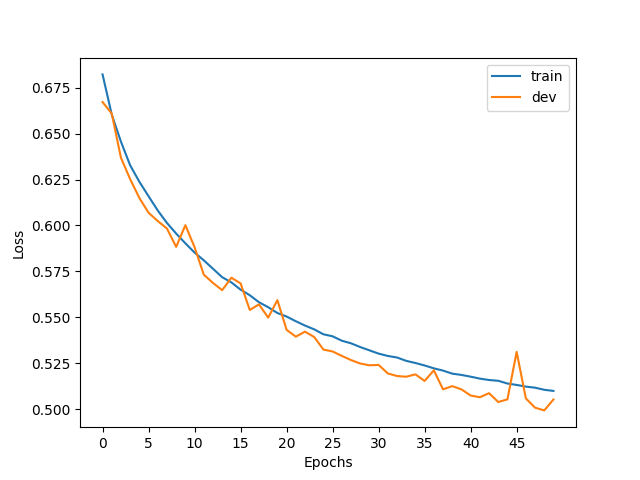
\includegraphics[width=0.45\textwidth]{gradient_descent_loss.png}
   \caption{train and dev loss}
\end{figure}\\


\bibliographystyle{apalike}
\bibliography{ref}

\end{document}